\documentclass[serif]{beamer}
\usepackage{mathpazo}  
\usepackage{pdfpages}
\usepackage{listofsymbols}
\usepackage{multirow}
%\usepackage[pdftex]{hyperref}
\usepackage[dutch,english]{babel}
\usepackage{tikz}
%%\usepackage{mathdesign}
\usepackage{wrapfig}
%%\usepackage{picins} %plaatjes naast text
\usepackage{color}
\usepackage{enumerate}
%%\usepackage{enumitem}
\usepackage{paralist}
\usepackage{framed}
\usepackage{fancybox} %kaders

\usepackage{amsmath,amssymb,mathrsfs}
\usepackage{amsthm}
\usepackage{wasysym}
%\usepackage{extarrows}
\setlength{\parindent}{0pt}






\begin{document}
\begin{frame}{}

\begin{center}
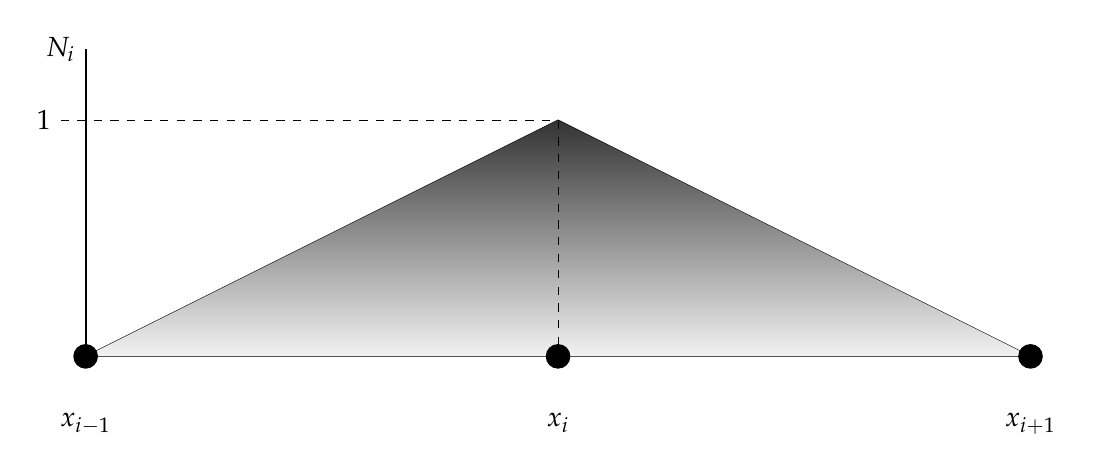
\begin{tikzpicture}[scale=3.0]
    % Draw axes
    \draw [-,thick] (0,1.3) node (yaxis) [left] {$N_i$}
        |- (4,0) node (xaxis) [right] {};
    % Draw two intersecting lines
    \draw (0,0) coordinate (a_1) -- (2,1) coordinate (a_2);
    \draw (2,1) coordinate (b_1) -- (4,0) coordinate (b_2);
    \draw (2,0) coordinate (b_3);
    \draw (0,-0.2) node[below] {$x_{i-1}$};
    \draw (2,-0.2) node[below] {$x_{i}$};
    \draw (4,-0.2) node[below] {$x_{i+1}$};
    
 \shade[bottom color=gray!10, top color=black!80] (0,0) --(2,0) --(2,1);
 \shade[bottom color=gray!10, top color=black!80] (4,0) --(2,0) --(2,1);

\node[draw,circle,inner sep=3pt,fill] at (b_3) {};
\node[draw,circle,inner sep=3pt,fill] at (b_2) {};
\node[draw,circle,inner sep=3pt,fill] at (a_1) {};

\draw[dashed] (yaxis |- b_1) node[left] {$1$}
        -| (xaxis -| b_1) node[below] {};

\end{tikzpicture}
\end{center}
\end{frame}



\end{document}